\documentclass[a4paper]{article}
\usepackage[utf8]{inputenc}
\usepackage{eso-pic}
\usepackage{smartdiagram}
\usepackage{amssymb}
\usepackage[ngerman]{babel}
\usepackage{qrcode}
\usepackage{wrapfig}
\usepackage{hyperref}
\usepackage{cite}
\usepackage{halloweenmath}

\definecolor{ipt-DARK-blue}{RGB}{0,39,59}
\definecolor{ipt-dark-blue}{RGB}{0,78,122}
\definecolor{ipt-blue}{RGB}{0,101,160}
\definecolor{ipt-light-blue}{RGB}{92,179,230}
\definecolor{ipt-LIGHT-blue}{RGB}{213,235,242}
\definecolor{ipt-DARK-red}{RGB}{102,25,50}
\definecolor{ipt-dark-red}{RGB}{181,0,58}
\definecolor{ipt-red}{RGB}{233,0,75}
\definecolor{ipt-light-red}{RGB}{247,57,74}
\definecolor{ipt-LIGHT-red}{RGB}{242,208,213}
\definecolor{ipt-green}{RGB}{64,183,183}
\definecolor{ipt-light-green}{RGB}{149,219,219}
\definecolor{ipt-LIGHT-green}{RGB}{199,237,237}
\definecolor{ipt-grey}{RGB}{144,150,153}
\definecolor{ipt-light-grey}{RGB}{192,200,204}

\hypersetup{colorlinks=true,linkcolor=ipt-blue,urlcolor=ipt-blue}

\title{\textbf{Building a Deployment Pipeline in three steps} \\ \vspace{.5cm} \qrcode{http://www.ipt.ch}
}

\author{Bastian Bukatz  $\bigskull$}



\newcommand\BackgroundPic{%
\put(0,0){%
\parbox[b][\paperheight]{\paperwidth}{%
\vfill

\includegraphics[width=\paperwidth,height=\paperheight,keepaspectratio]{pictures/ipt_titelpage2.jpg}%
}}}


\begin{document}
\AddToShipoutPicture{\BackgroundPic}
\maketitle


\begin{abstract}
Dieses Dokument beschreibt ein Vorgehen zum Aufbau einer Deplyoment Pipeline in drei Schritten.
\vspace{.5cm}
\centering
\smartdiagramset{
  planet size=2cm,
  planet color = none,
  border color=black,sequence item border color=none,sequence item font size=\footnotesize, sequence item text color=ipt-blue,
  set color list={ipt-light-grey,ipt-light-green,ipt-light-blue}
}
\smartdiagram[sequence diagram]{Run,Verify,Release}
\end{abstract}

\section*{Was ist eine Deployment Pipeline}

\begin{wrapfigure}{l}{0pt}
\begin{tikzpicture}[]
%3D-Koordinatensystem:
\draw[thick,ipt-grey,->, >=latex] (0,0,0) -- (2,0,0) node[below]{$Reichweite$};
\draw[thick,ipt-grey,->, >=latex] (0,0,0) -- (0,2,0) node[left]{$Inhalt$};
\draw[thick,ipt-grey,->, >=latex] (0,0,0) -- (0,0,2) node[left]{$Features$};
\filldraw[color=ipt-light-grey, semitransparent] (1,0,0) -- (0,.5,0) -- (0,0,.5) -- cycle;
\filldraw[color=ipt-light-green, semitransparent] (1.3,0,0) -- (0,1.2,0) -- (0,0,1.5) -- cycle;
\filldraw[color=ipt-light-blue, semitransparent] (1.8,0,0) -- (0,1.8,0) -- (0,0,1.8) -- cycle;
\end{tikzpicture}
\end{wrapfigure}
Die Aufgabe der Deployment Pipeline besteht darin, Änderungen zu erkennen, die zu Problemen in der Produktion führen. Dazu gehören Probleme bezüglich der Performance, Sicherheit oder Benutzerfreundlichkeit. In einer Deplyoment Pipeline werden dazu alle nötigen Schritte nacheinander von Links nach Rechts durchlaufen. Man spricht daher, wenn es darum geht Feedback über mögliche Prolbeme in Produktion möglichst früh zu erhalten, von Left-Shift.




\subsection*{Umfang}
Der Umfang einer Deplyoment Pipeline kann in drei Dimensionen beschrieben werden.
\begin{description}
  \item[Reichweite] \textit{Wie lang ist die Pipeline.} Gehts sie vom Sourcecode bis in Produktion oder nur in eine nicht integrierte Testumgebung?
  \item[Inhalt] \textit{Was fliesst durch die Pipeline?} Wird nur der Sourcecode der Application durch die Pipeline behandelt, oder auch Konfiguration sowie der Aufbau der Infrastruktur?
  \item[Features] \textit{Welche Ventile hat die Pipeline?} Wird nur gebaut und deployed? Werden Tests ausgefürht? Welche? Werden Security-Checks ausgeführt? Werden Metriken über Test-Coverage oder Performance Daten erhoben?
\end{description}

\begin{center}
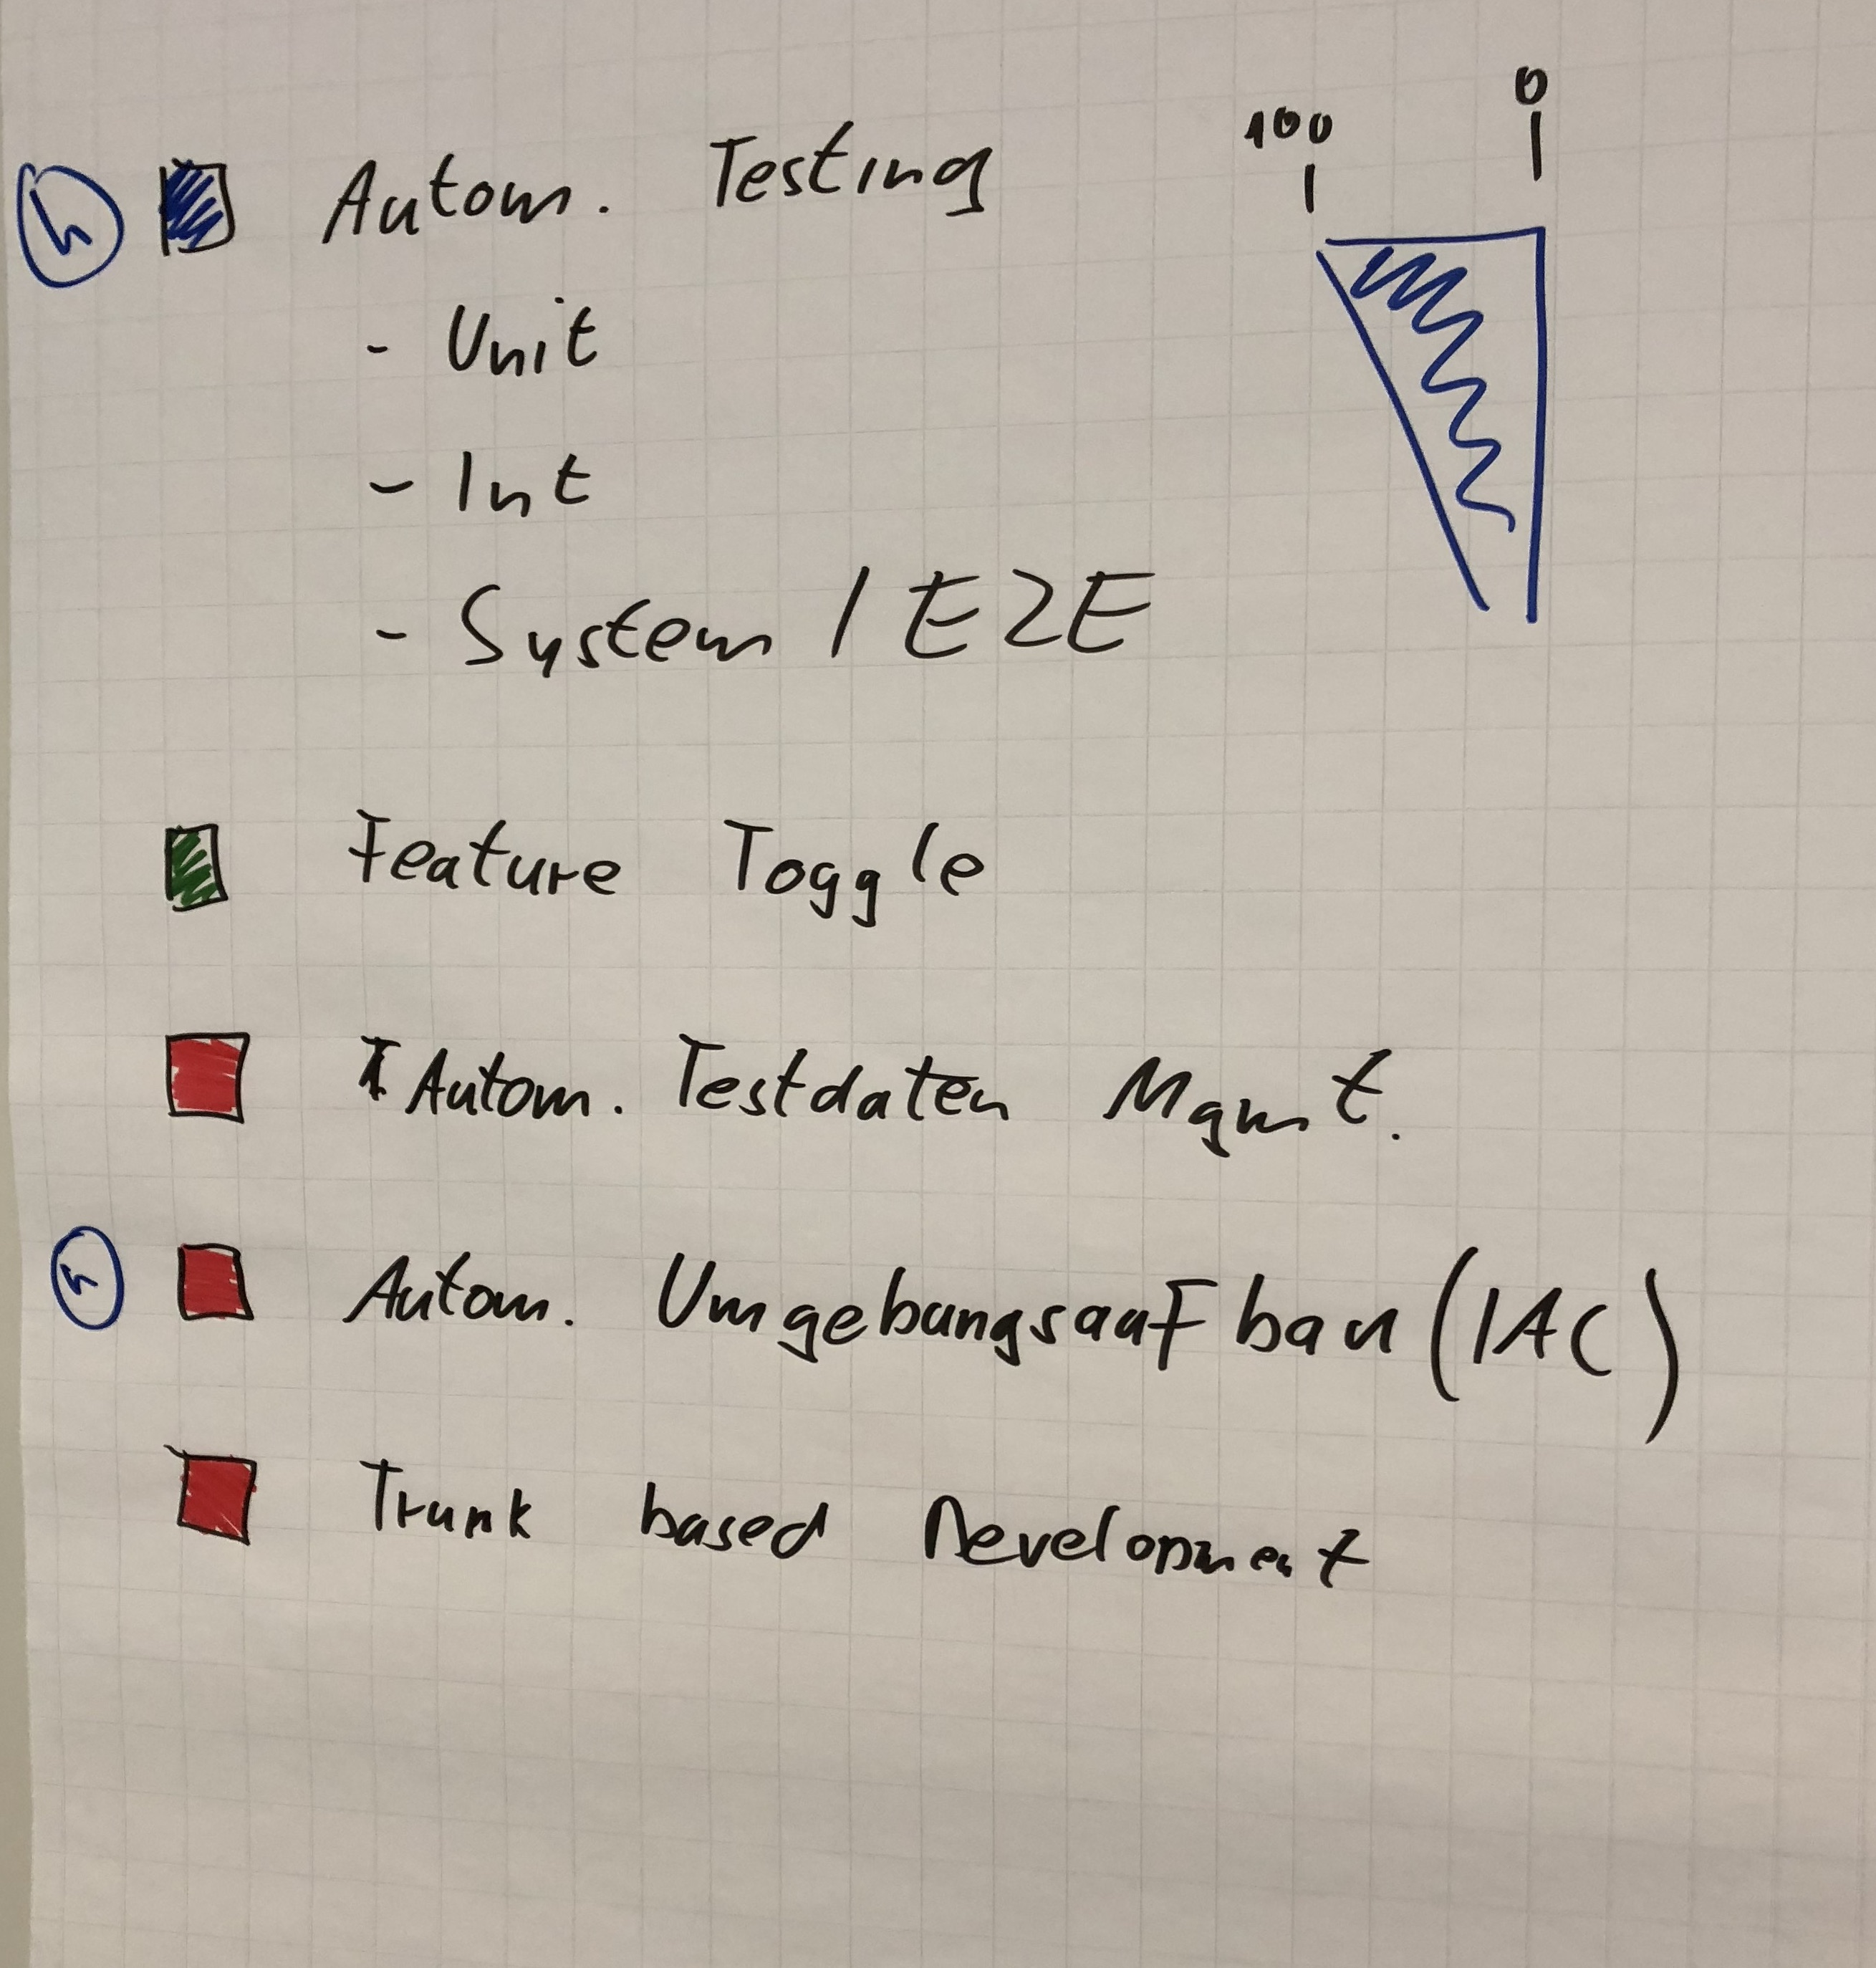
\includegraphics[width=0.5\paperwidth,keepaspectratio]{pictures/ScopeDPmyHelsana.jpg}
\end{center}


\section*{myHelsana}
\begin{itemize}
  \item[\textcolor{ipt-light-blue}{$\blacksquare$}] Automatisiertes Testing
  \begin{itemize}
    \item[] Unit Testing
    \item[] Integration Testing
    \item[] System / e2e Testing
  \end{itemize}
  \item[\textcolor{ipt-green}{$\blacksquare$}] Feature Toggles
  \item[\textcolor{ipt-light-red}{$\blacksquare$}] Automatisiertes Testdaten Management
  \item[\textcolor{ipt-light-red}{$\blacksquare$}] Automatisierter Umgebungsaufbau (IAC)
  \item[\textcolor{ipt-light-red}{$\blacksquare$}] Trunk based Development
\end{itemize}

\subsection*{Step 1}
Aufbau einer funktionierenden Deployment Pipeline.
Länge: Source to System Integration
Inhalt: Sourcecode, Konfiguration, (Infrastruktur)
Features: Bestehende Tests. Unit / Ingetration / e2e

\subsection*{Step 2}
Aufbau einer funktionierenden Deployment Pipeline.
\begin{description}
  \item[Länge:] Source to System Integration. Push Button Deployment in Produktion.
  \item[Inhalt:] Sourcecode, Konfiguration, Infrastruktur
  \item[Features:] Ausbau Testing, Ausbau Metriken, Performance, Security ...
\end{description}

\subsection*{Step 3}
Wenn die der Feature Umfang der Deployment Pipeline ausreichend ist um eine produktionsreive Qualität zu garantieren kann direkt automatisiert in Produktion deployed werden.
Länge: Source to System Integration
Inhalt: Sourcecode, Konfiguration, Infrastruktur
Features: Ausbau Testing, Ausbau Metriken, Performance, Security ...

\subsection*{Trunk based Development}
Resultat der ersten Phase ist eine erste funktionierende Deplyoment Pipeline
mit minimaler Ausdehung bezüglich der beiden Dimensionen Reichweite und Inhalt.

\section*{Ressources}
\begin{itemize}
  \item \href{http://www.informit.com/articles/article.aspx?p=1833567}{Four Principles of Low-Risk Software Releases}
  \item \href{http://www.informit.com/articles/article.aspx?p=1621865&seqNum=8}{Continuous Delivery: Anatomy of the Deployment Pipeline; Jez Humble, }
\end{itemize}

\cite{Lewin2015}
\cite{Humble2012a}
\cite{Humble2010}
\cite{Burnes2004}

\newpage
\bibliography{library}
\bibliographystyle{alphadin}

\end{document}
